\documentclass[preprint,12pt]{elsarticle}

\usepackage[T1]{fontenc}
\usepackage[utf8]{inputenc}
\usepackage{lmodern}
\usepackage[protrusion=true,expansion=false]{microtype}
\DisableLigatures{encoding = T1, family = *}
\usepackage{graphicx}
\usepackage{booktabs}
\usepackage{amsmath}
\usepackage{siunitx}
\usepackage{xcolor}
\usepackage[hidelinks]{hyperref}

\journal{Computers \& Geosciences}

% Replace these three placeholders after creating the GitHub repository and
% the Zenodo archive.
\newcommand{\codeurl}{https://github.com/L-peak/gwbench}
\newcommand{\zenododoi}{https://doi.org/10.5281/zenodo.23749304}
\newcommand{\kaggleurl}{https://www.kaggle.com/code/kkksssaaalzy/gwbench-gru-h30}

\begin{document}

\begin{frontmatter}

\title{When Does Deep Learning Beat Persistence for Groundwater-Level Forecasting? A Reproducible Benchmark and a Persistence-Anchored Residual Model}

\author{Zhaoyang Li\corref{cor1}}
\ead{3286533389@qq.com}
\affiliation{organization={Henan Polytechnic University}, city={Jiaozuo}, state={Henan}, country={China}}

\cortext[cor1]{Corresponding author.}

\begin{abstract}
Groundwater-level forecasting is increasingly tackled with deep learning, but
reported gains are difficult to compare because studies use different wells,
splits, horizons, and baselines. We present \texttt{gwbench}, a reproducible
benchmark built from public USGS National Water Information System daily
depth-to-water records for 279 wells in California, Nebraska, and Texas
(2000--2024), with a 74-well clean core and standardized temporal splits. We
evaluate persistence, seasonal naive, per-site ridge regression, and a global
residual GRU. Persistence is extremely strong at short horizons (mean NSE 0.97
at one day), and a calibrated residual GRU is statistically tied with
persistence at 30 days. At 90 days, it improves median NSE from $-0.18$ to $0.27$ (95\% CI for the
median gain 0.03--0.21) and mean KGE from 0.46 to 0.51, although mean NSE and
mean KGE confidence intervals include zero and one distribution-shift well
dominates the mean. A per-site validation-fitted blending weight is essential:
the uncalibrated GRU fails catastrophically on low-variance wells. Performance remains stable
when 10--50\% of input observations are masked. The benchmark, code, and
experiment configurations are released to support reproducible comparison.
\end{abstract}

\begin{keyword}
groundwater \sep machine learning \sep benchmark \sep persistence \sep
forecasting \sep reproducibility
\end{keyword}

\end{frontmatter}

\section{Introduction}

Groundwater is a primary water source for agriculture, ecosystems, and
municipal supply, and water-level observations are among the most direct
indicators of aquifer stress. Machine-learning (ML) models are now widely used
to forecast groundwater levels, often with recurrent or attention-based
architectures \citep{hochreiter1997,cho2014,kratzert2019,shen2018,khan2023,dey2025}. Reported
gains, however, are hard to compare: studies differ in well selection,
train/test splitting, forecast horizon, and---critically---the strength of the
baseline. Random train/test splits can leak information across nearby dates,
and persistence (the last observed value) is rarely reported even though it is
extremely competitive for slow-moving hydrological variables.

This paper makes four contributions. First, we release a reproducible benchmark
for daily groundwater-level forecasting built entirely from public USGS data,
with temporal splits and a documented quality-control (QC) pipeline. Second, we
quantify the skill of persistence from 1 to 180 days on a common panel,
exposing where ML can and cannot add value. Third, we show that a global
residual GRU with site embeddings still fails catastrophically on low-variance
wells, and that a per-site validation-fitted persistence blending weight fixes
this failure. Fourth, we report a horizon-dependent conclusion that is usually
missing from the literature: at 30 days the calibrated model is statistically
tied with persistence on mean NSE, whereas at 90 days it improves median NSE,
mean KGE, and median KGE across seeds. We also show that the calibrated model
is robust to 10--50\% missing input observations.

We position this work as a benchmark and reproducibility study rather than a
new network architecture. Recent reviews document the rapid growth of
groundwater-level ML \citep{khan2023}; our contribution is the combination of
an open, standardized pipeline, honest evaluation against persistence, and
practical guidance for when a simple residual model does---and does not---beat
a strong baseline. Residual forecasting and persistence blending are known
techniques; the novelty is the benchmark protocol and the empirical
characterization of failure modes, not a new algorithm.

\section{Data}

\subsection{USGS records and selection}

All observations come from the USGS National Water Information System (NWIS)
\citep{usgs2026}. We use parameter code 72019 (depth to water level, feet below
land surface) and statistic code 00001 (daily maximum). Wells are selected from
California, Nebraska, and Texas---the states with the largest number of long
daily records in our initial catalog scan---subject to three criteria: at least
3,650 observations, a first-to-last span of at least 10 years, and a record
extending to at least 2015. The final collection contains 279 wells and
1,581,469 observed daily values from 2000--2024.

\subsection{Panels and quality control}

We build a complete daily panel for each site and mark observed versus missing
days explicitly. Three panels are used (Table~\ref{tab:panels}): the full set,
a core set with at least 70\% observed coverage, and a clean core that also
removes wells with more than five day-to-day jumps larger than 5 ft. Sentinel
values (100000.x) are removed before panel construction. We flag rather than
silently correct jumps and long gaps, because they may reflect real datum or
sensor changes. All main experiments use the clean core; the full and screened
core panels are provided for extension and stress testing.

\begin{table}[t]
\centering
\caption{Benchmark panels. Observed days are the number of non-missing daily
values in the panel. The clean core is the primary analysis set; the full and
screened core panels are provided for extension and stress testing.}
\label{tab:panels}
\begin{tabular}{lrrrl}
\toprule
Panel & Wells & Panel rows & Observed days & Selection rule \\
\midrule
Full & 279 & 2,547,828 & 1,581,469 & all selected wells \\
Core (screened) & 89 & 812,748 & 664,435 & coverage $\geq 70\%$ \\
Clean core (main) & 74 & 675,768 & 556,449 & core, $\leq 5$ jumps $>5$ ft \\
\bottomrule
\end{tabular}
\end{table}

\begin{figure}[t]
\centering
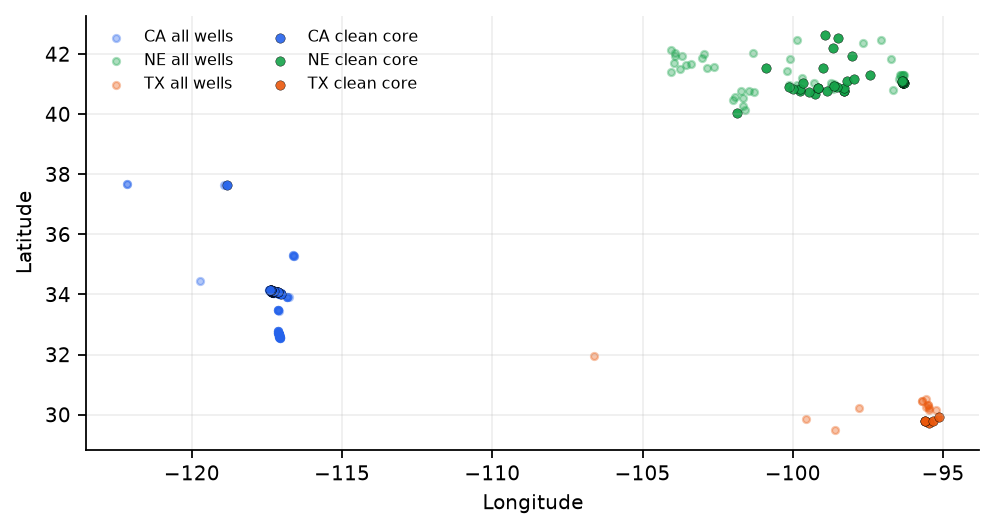
\includegraphics[width=\linewidth]{figures/fig1_study_map.png}
\caption{Locations of the 279 selected USGS wells. Light markers show all
wells; dark markers show the 74-well clean core used for the main experiments.}
\label{fig:map}
\end{figure}

\begin{figure}[t]
\centering
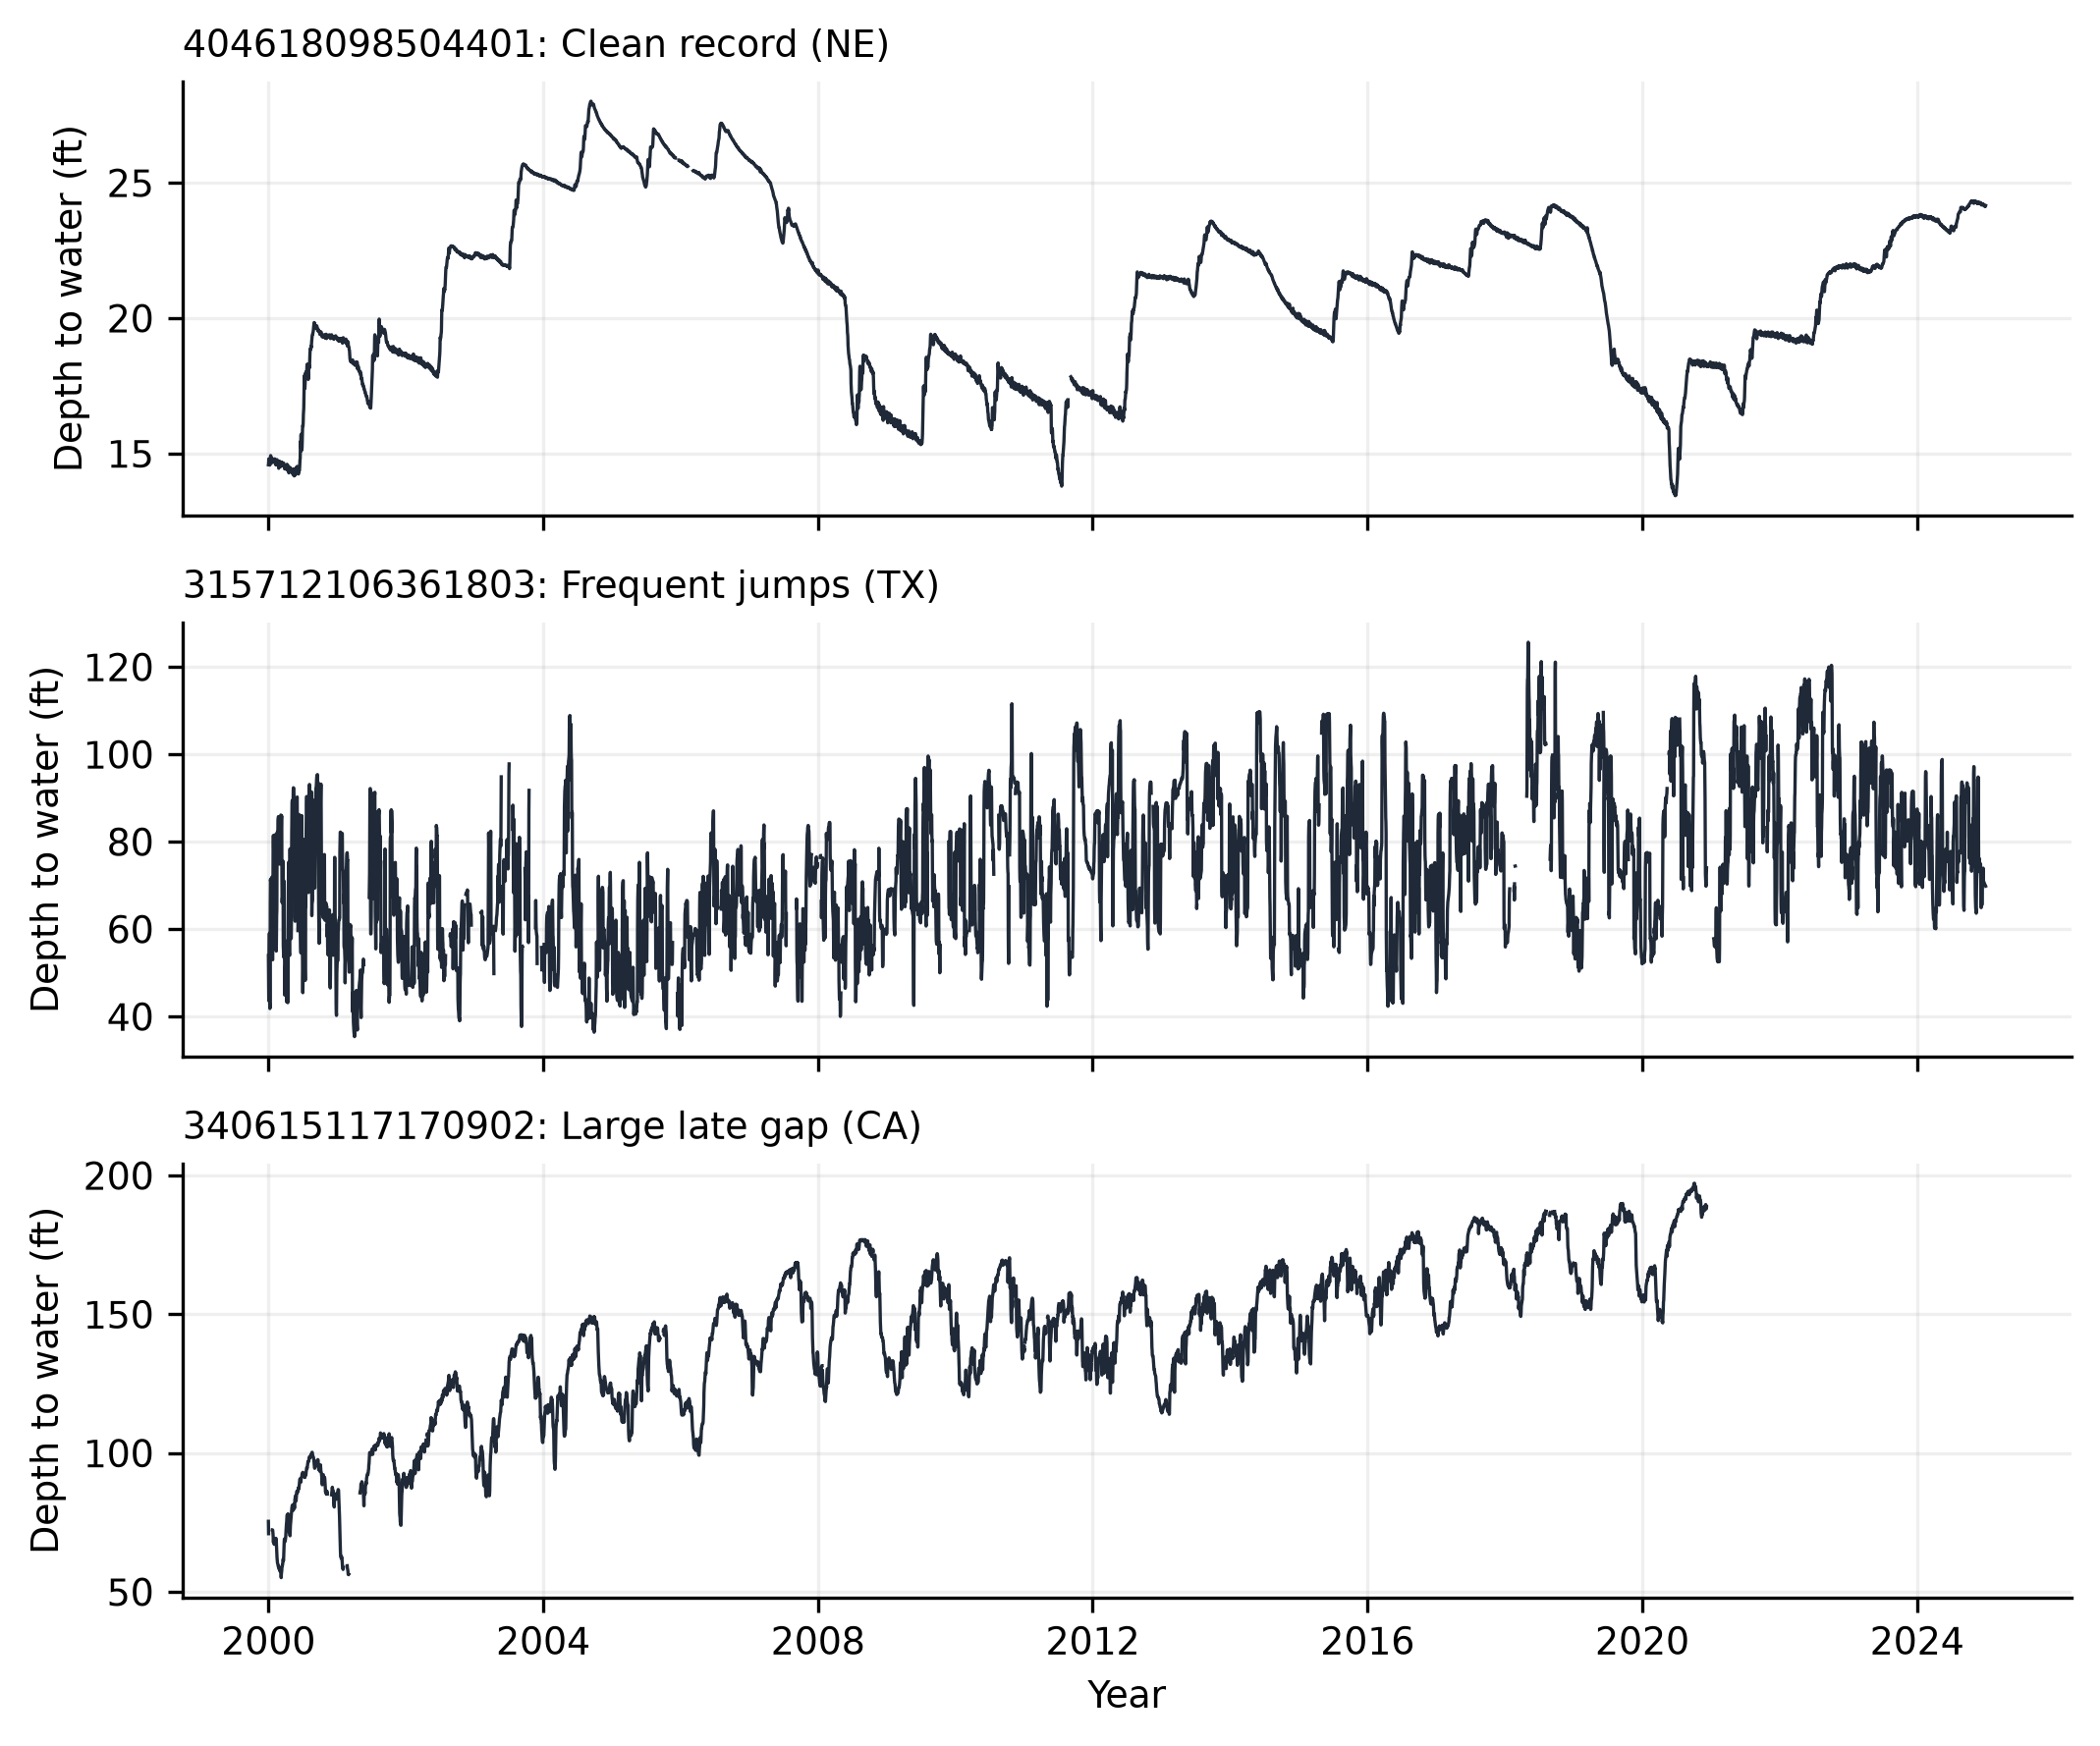
\includegraphics[width=\linewidth]{figures/fig2_examples.png}
\caption{Representative daily records: a clean Nebraska well (top), a Texas
well with frequent short-term jumps (middle), and a California well with a
large late-record gap (bottom).}
\label{fig:examples}
\end{figure}

\section{Methods}

\subsection{Splits}

We use a strict temporal split: training data through 2015, validation data
2016--2018, and test data 2019--2024. The validation period is used for early
stopping and for fitting the per-site blending weight; the test period is
never used for model selection or calibration.

\subsection{Baselines}

\textbf{Persistence} predicts the last observed value before the forecast
anchor. \textbf{Seasonal naive} predicts the value 365 days before the target
date. A \textbf{per-site ridge regression} uses the last value, rolling means
(7, 30, 90, 365 days), rolling standard deviations, and day-of-year sine/cosine
features; a linear time trend is excluded to reduce extrapolation. Ridge is
reported as a secondary learned baseline.

\subsection{Global residual GRU}

The main model is a two-layer GRU \citep{cho2014} shared across wells. Each
input window spans 365 days and contains three channels: the normalized value,
an observation mask, and day-of-year sine/cosine features. A learned site
embedding is concatenated to every time step. The target is the residual from
the last observed value in the window:
\begin{equation}
  y_{\text{res}} = \frac{y_{t+h} - \mu_s}{\sigma_s}
  - \frac{y_{\text{last}} - \mu_s}{\sigma_s},
\end{equation}
where $\mu_s$ and $\sigma_s$ are the training-period mean and standard deviation
of site $s$. Site-wise z-scoring is used instead of a global scale because wells
differ by orders of magnitude in depth and variance; a global scale would let
deep, high-variance wells dominate the MSE. The residual target is
dimensionless, so the same model can be trained across sites. This forces a
zero output to reproduce persistence and lets the model learn only the
correction. We use hidden size 64, dropout 0.2, Adam with
learning rate $10^{-3}$, batch size 256, MSE loss, gradient clipping, and early
stopping on validation RMSE. Training anchors use a stride of three days; test
anchors use every day.

\subsection{Persistence blending}

For each site, we fit a scalar $\alpha_s \in [0,1]$ on validation predictions:
\begin{equation}
  \hat{y}_{\text{cal}} = \hat{y}_{\text{pers}} +
  \alpha_s \left(\hat{y}_{\text{GRU}} - \hat{y}_{\text{pers}}\right).
\end{equation}
The closed-form least-squares solution is clipped to $[0,1]$; a site whose GRU
is worse than persistence receives $\alpha_s=0$ and falls back to persistence.
This step uses validation data only and is applied unchanged to all test
periods and missingness levels.

\subsection{Metrics and robustness tests}

We report RMSE, MAE, Nash--Sutcliffe efficiency (NSE)
\citep{nash1970}, and Kling--Gupta efficiency (KGE) \citep{gupta2009}, as both
mean and median across wells. We also report the fraction of wells on which the
model beats persistence (win rate) and a paired bootstrap over wells for the
mean difference in NSE and KGE. Main results are averaged over seeds 1--3.
For the missing-data stress test, we randomly hide 10\%, 30\%, or 50\% of the
observed input values at test time without retraining.

\section{Results}

\subsection{Persistence is strong at short horizons}

Table~\ref{tab:persistence} and Figure~\ref{fig:horizon} show persistence skill
on the clean core using the same anchor protocol as the model. Mean NSE falls
from 0.974 at one day to 0.573 at 30 days and $-0.218$ at 90 days. Median NSE
is 0.729 at 30 days and $-0.181$ at 90 days. Seasonal naive is worse than
persistence at every horizon (mean NSE $-3.16$).

\begin{table}[t]
\centering
\caption{Persistence skill on the 74-well clean core using the model anchor
protocol. The number of evaluated wells is 74 for horizons up to 30 days and
73 for 90 and 180 days.}
\label{tab:persistence}
\resizebox{\linewidth}{!}{%
\begin{tabular}{rrrrrr}
\toprule
Horizon (d) & NSE mean & NSE median & KGE mean & KGE median & RMSE mean \\
\midrule
1   &  0.974 &  0.993 & 0.984 & 0.996 & 0.231 \\
7   &  0.867 &  0.966 & 0.927 & 0.967 & 0.691 \\
30  &  0.573 &  0.729 & 0.784 & 0.823 & 1.759 \\
90  & -0.218 & -0.181 & 0.456 & 0.463 & 3.773 \\
180 & -1.746 & -1.363 & 0.063 & 0.076 & 5.532 \\
\bottomrule
\end{tabular}}
\end{table}

\begin{figure}[t]
\centering
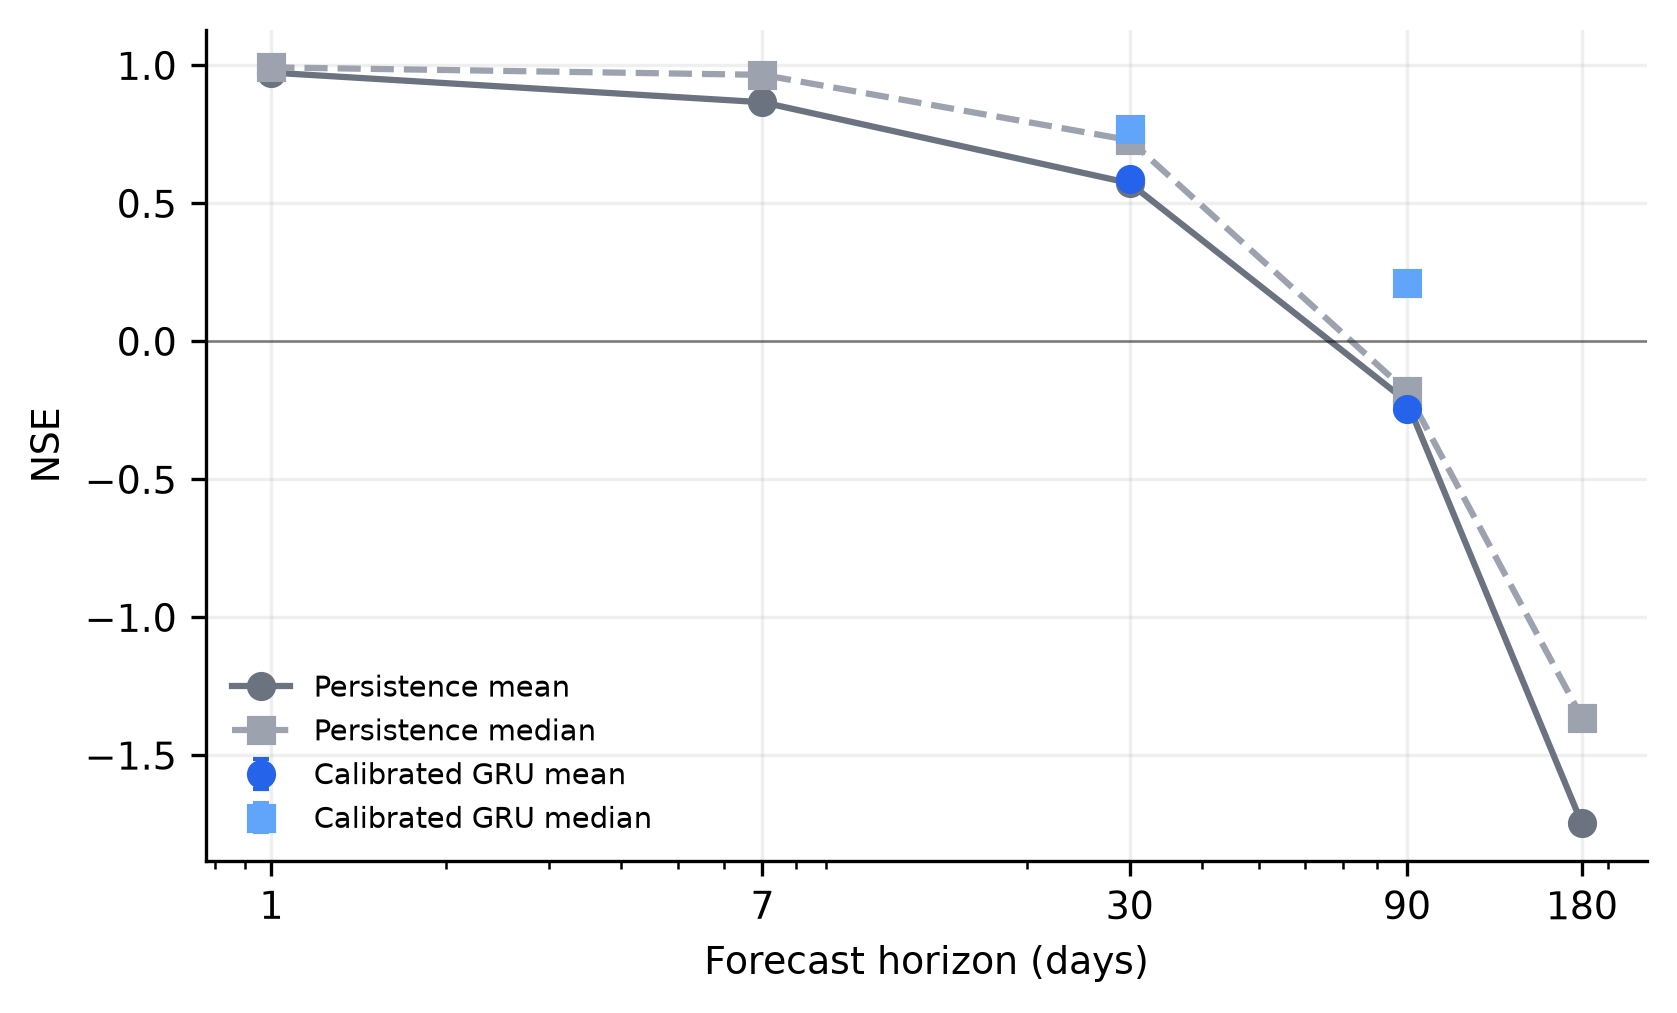
\includegraphics[width=0.8\linewidth]{figures/fig3_horizon_skill.png}
\caption{Persistence skill versus forecast horizon, with calibrated GRU results
at 30 and 90 days (mean $\pm$ standard deviation over seeds 1--3).}
\label{fig:horizon}
\end{figure}

\subsection{30 days: a statistical tie with persistence}

Table~\ref{tab:models} summarizes the 30- and 90-day results. At 30 days the
raw residual GRU has a median NSE of 0.564 but a mean NSE of $-3.155$ because
of a few catastrophic wells. Calibration removes these failures and yields a
mean NSE of $0.575 \pm 0.012$ versus 0.573 for persistence; the paired
bootstrap 95\% confidence interval for mean $\Delta$NSE is $[-0.077, 0.052]$,
so the mean difference is not statistically distinguishable from zero. Median
NSE improves from 0.729 to $0.765 \pm 0.010$, but mean KGE is slightly lower
($0.761 \pm 0.007$ vs 0.784). We therefore describe the 30-day result as a tie
on mean NSE, not as an ML win. Seed-averaged per-site changes are mostly small:
44/74 wells have positive $\Delta$NSE, 28 negative, and 2 zero; the median
$\Delta$NSE is $+0.007$ (95\% CI $0.000$--$0.018$), while the mean is $+0.002$
(95\% CI $-0.077$--$0.052$). The mean $\Delta$KGE is $-0.023$ (95\% CI
$-0.053$--$-0.001$), and the median is $-0.002$ (95\% CI $-0.011$--$0.001$).
This confirms that the 30-day result is a tie, not a win.

\begin{table}[t]
\centering
\caption{Forecast skill on the clean core. Values are mean $\pm$ standard
deviation over seeds 1--3 for the neural models; persistence is deterministic.
The persistence rows use the same evaluation anchors as the models.}
\label{tab:models}
\resizebox{\linewidth}{!}{%
\begin{tabular}{llrrrr}
\toprule
Horizon & Model & NSE mean & NSE median & KGE mean & KGE median \\
\midrule
30 d & Persistence & 0.573 & 0.729 & 0.784 & 0.823 \\
30 d & Raw GRU & $-3.155 \pm 1.320$ & $0.564 \pm 0.028$ & $0.443 \pm 0.063$ & $0.761 \pm 0.022$ \\
30 d & Calibrated GRU & $0.575 \pm 0.012$ & $0.765 \pm 0.010$ & $0.761 \pm 0.007$ & $0.838 \pm 0.009$ \\
\midrule
90 d & Persistence & $-0.218$ & $-0.181$ & 0.456 & 0.463 \\
90 d & Raw GRU & $-14.169 \pm 7.688$ & $-0.013 \pm 0.195$ & $0.086 \pm 0.033$ & $0.492 \pm 0.024$ \\
90 d & Calibrated GRU & $-0.189 \pm 0.093$ & $0.267 \pm 0.022$ & $0.505 \pm 0.014$ & $0.585 \pm 0.021$ \\
\bottomrule
\end{tabular}}
\end{table}

\subsection{Ridge baseline}

A per-site ridge regression with lag and rolling features (last value, 7/30/90/
365-day means and standard deviations, and day-of-year terms; no linear time
trend) was evaluated on exactly the same test anchors as the GRU. It achieved
median NSE 0.780 at 30 days and 0.304 at 90 days, compared with persistence
0.729 and $-0.181$. Its mean NSE was 0.264 at 30 days and $-1.688$ at 90 days,
showing that even a linear model can be dominated by a few trending or
low-variance wells. Median KGE was 0.847 and 0.622, compared with 0.822 and
0.462 for persistence. The ridge baseline therefore improves the median but is
not robust in the mean, reinforcing our emphasis on median and KGE.

\subsection{90 days: robust median and KGE gains}

At 90 days the calibrated model improves every aggregate point estimate
(Table~\ref{tab:models}), but the statistical support is strongest for the
median NSE. Median NSE rises from $-0.181$ to $0.267 \pm 0.022$,
mean KGE from 0.456 to $0.505 \pm 0.014$, and median KGE from 0.463 to
$0.585 \pm 0.021$. The NSE win rate is $49.7 \pm 3.8$ of 73 wells and the KGE
win rate is $41.0 \pm 3.6$ of 73. Seed-averaged per-site changes are asymmetric:
55/73 wells have positive $\Delta$NSE, 13 negative, and 5 zero; the median
$\Delta$NSE is $+0.115$ (95\% CI $0.033$--$0.207$), while the mean is $+0.029$
(95\% CI $-0.431$--$0.299$). The mean $\Delta$KGE is $+0.049$ (95\% CI
$-0.004$--$0.096$), and the median is $+0.019$ (95\% CI $0.000$--$0.036$).
The median NSE gain is the statistically robust result; the mean is sensitive
to a few wells. The mean NSE improvement is smaller and its
bootstrap interval includes zero because one well
(\texttt{413156098591201}) undergoes a validation-to-test shift: across seeds
its calibrated NSE ranges from $-13.27$ to $-17.33$, while persistence is
$-0.71$. Excluding that single well, the seed-averaged calibrated mean NSE is
$+0.013$ versus $-0.211$ for persistence (individual seeds range from
$-0.057$ to $+0.068$), and mean KGE is $0.524$ versus $0.457$. We therefore
treat median NSE and KGE as the robust 90-day result and report the outlier
explicitly.

\begin{figure}[t]
\centering
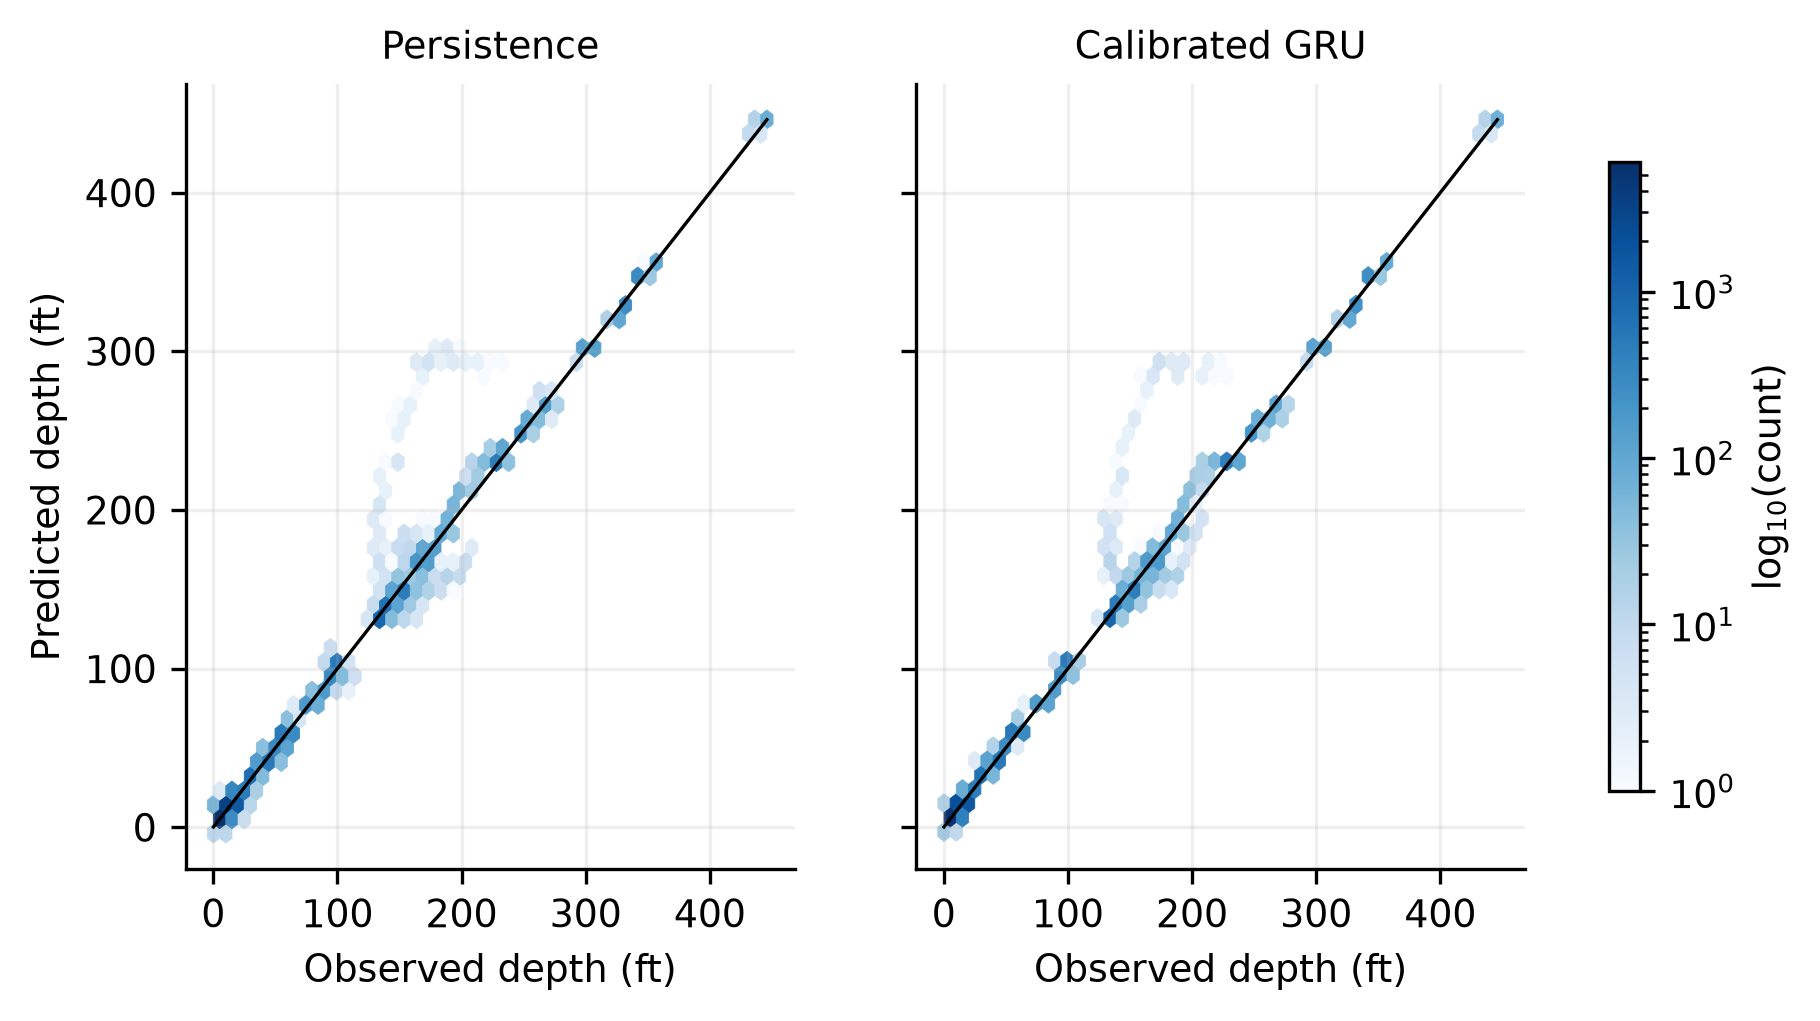
\includegraphics[width=\linewidth]{figures/fig4_scatter_h90.png}
\caption{Predicted versus observed 90-day depths on a random sample of test
anchors. Left: persistence; right: calibrated GRU. The diagonal is the 1:1
line.}
\label{fig:scatter}
\end{figure}

\subsection{Why calibration is necessary}

The raw GRU is unstable on low-variance wells. On 30-day forecasts its mean NSE
is $-3.155$ despite a median of 0.564; on 90-day forecasts the corresponding
values are $-14.169$ and $-0.013$. The per-site blending weight fixes this:
across seeds, $\alpha_s>0$ for 62--69 of 74 wells at 30 days and 58--67 of 74
wells at 90 days, with the remainder falling back to persistence
(Figure~\ref{fig:alpha}). The calibration is therefore not cosmetic; it is what
makes a global residual model usable across heterogeneous wells.

\begin{figure}[t]
\centering
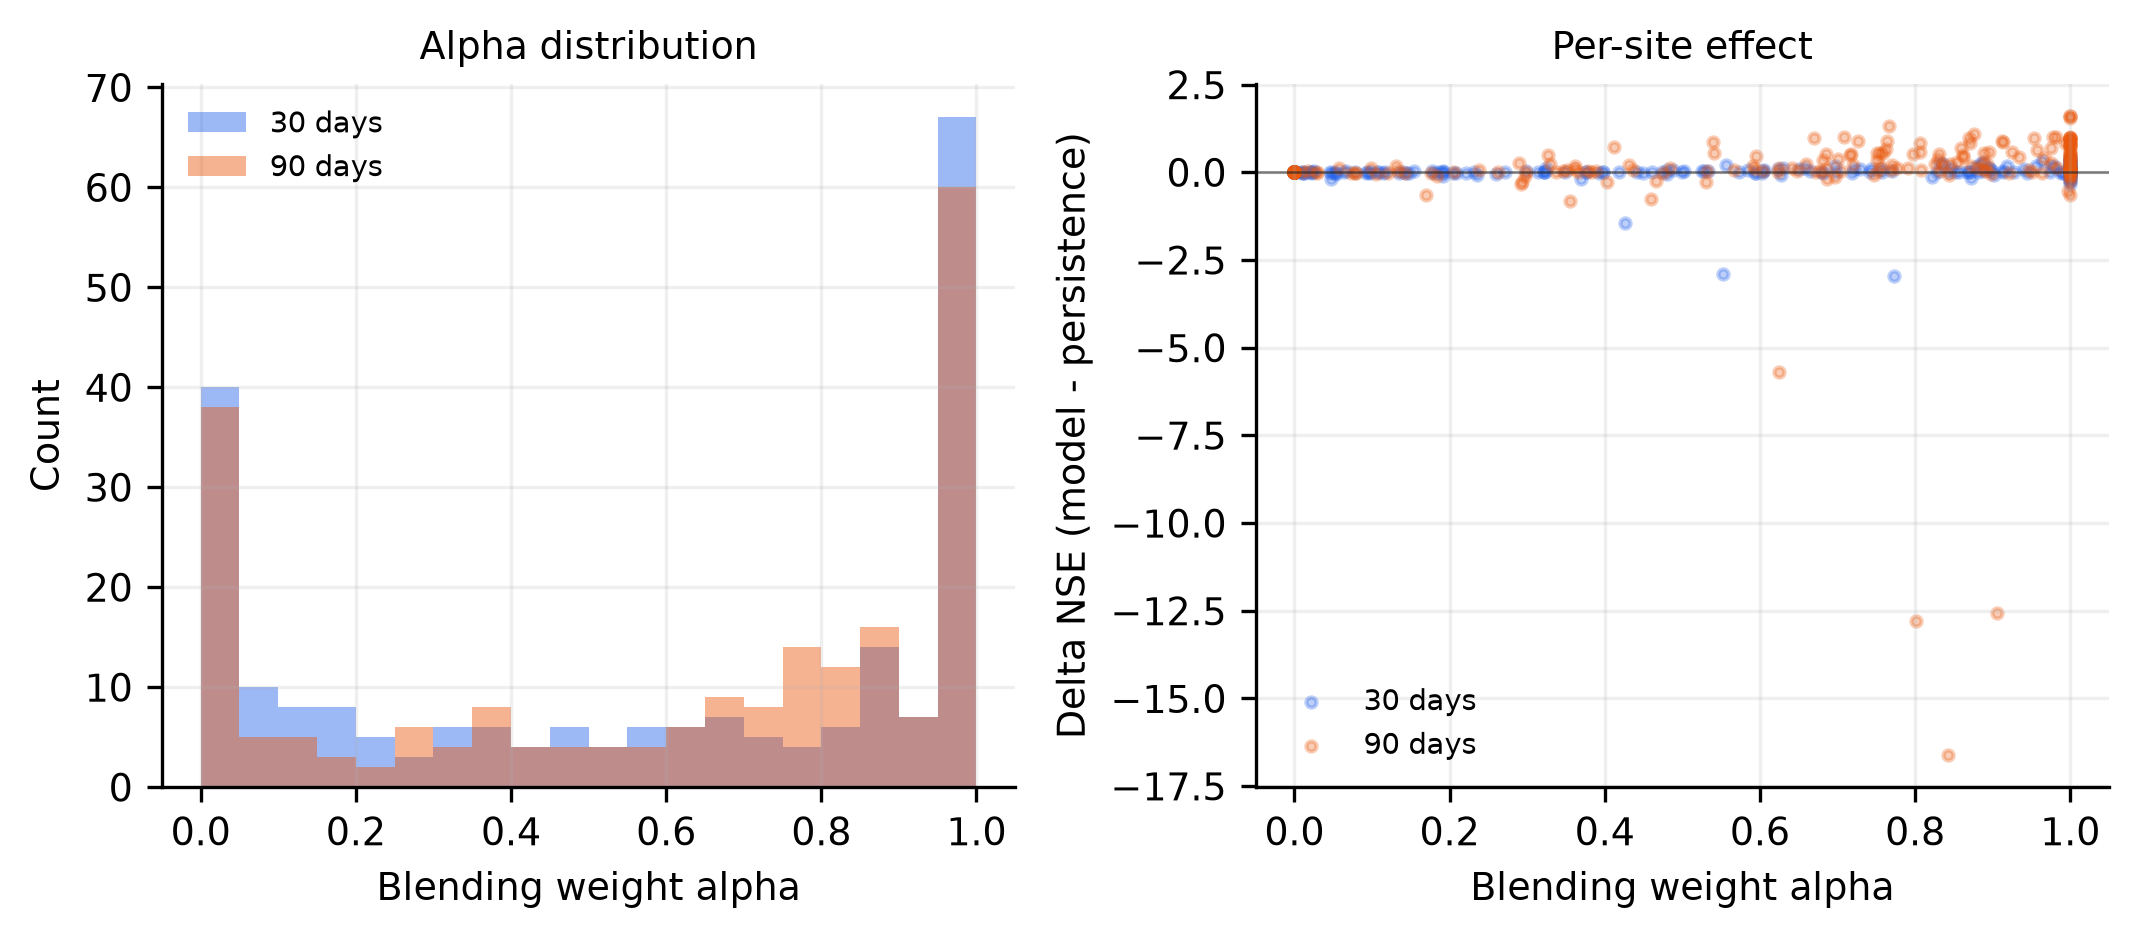
\includegraphics[width=\linewidth]{figures/fig5_alpha.png}
\caption{Distribution of the validation-fitted blending weight $\alpha_s$
(left) and its relationship to the per-site NSE difference on the test period
(right). Points below zero indicate wells where the calibrated model is worse
than persistence.}
\label{fig:alpha}
\end{figure}

\subsection{Missing-data robustness}

On a stride-7 test subset, hiding 10--50\% of the observed input values at test
time does not degrade performance (Table~\ref{tab:missing},
Figure~\ref{fig:missing}). At 30 days, mean NSE changes from 0.644 to 0.627 and
mean KGE from 0.777 to 0.787; at 90 days, mean NSE changes from 0.044 to 0.067
and mean KGE from 0.539 to 0.562. The stride-7 protocol is used for computational
tractability and is not directly comparable to the full test-set metrics in
Table~\ref{tab:models}; the relevant result is the flat trend across
missingness levels.

\begin{table}[t]
\centering
\caption{Missing-data stress test (no retraining). Values are means across
wells on a stride-7 test subset (every seventh test anchor); they are not
directly comparable to the full test set in Table~\ref{tab:models}.}
\label{tab:missing}
\begin{tabular}{rrrr}
\toprule
Horizon & Masked input & NSE mean & KGE mean \\
\midrule
30 d & 0\%  & 0.644 & 0.777 \\
30 d & 50\% & 0.627 & 0.787 \\
90 d & 0\%  & 0.044 & 0.539 \\
90 d & 50\% & 0.067 & 0.562 \\
\bottomrule
\end{tabular}
\end{table}

\begin{figure}[t]
\centering
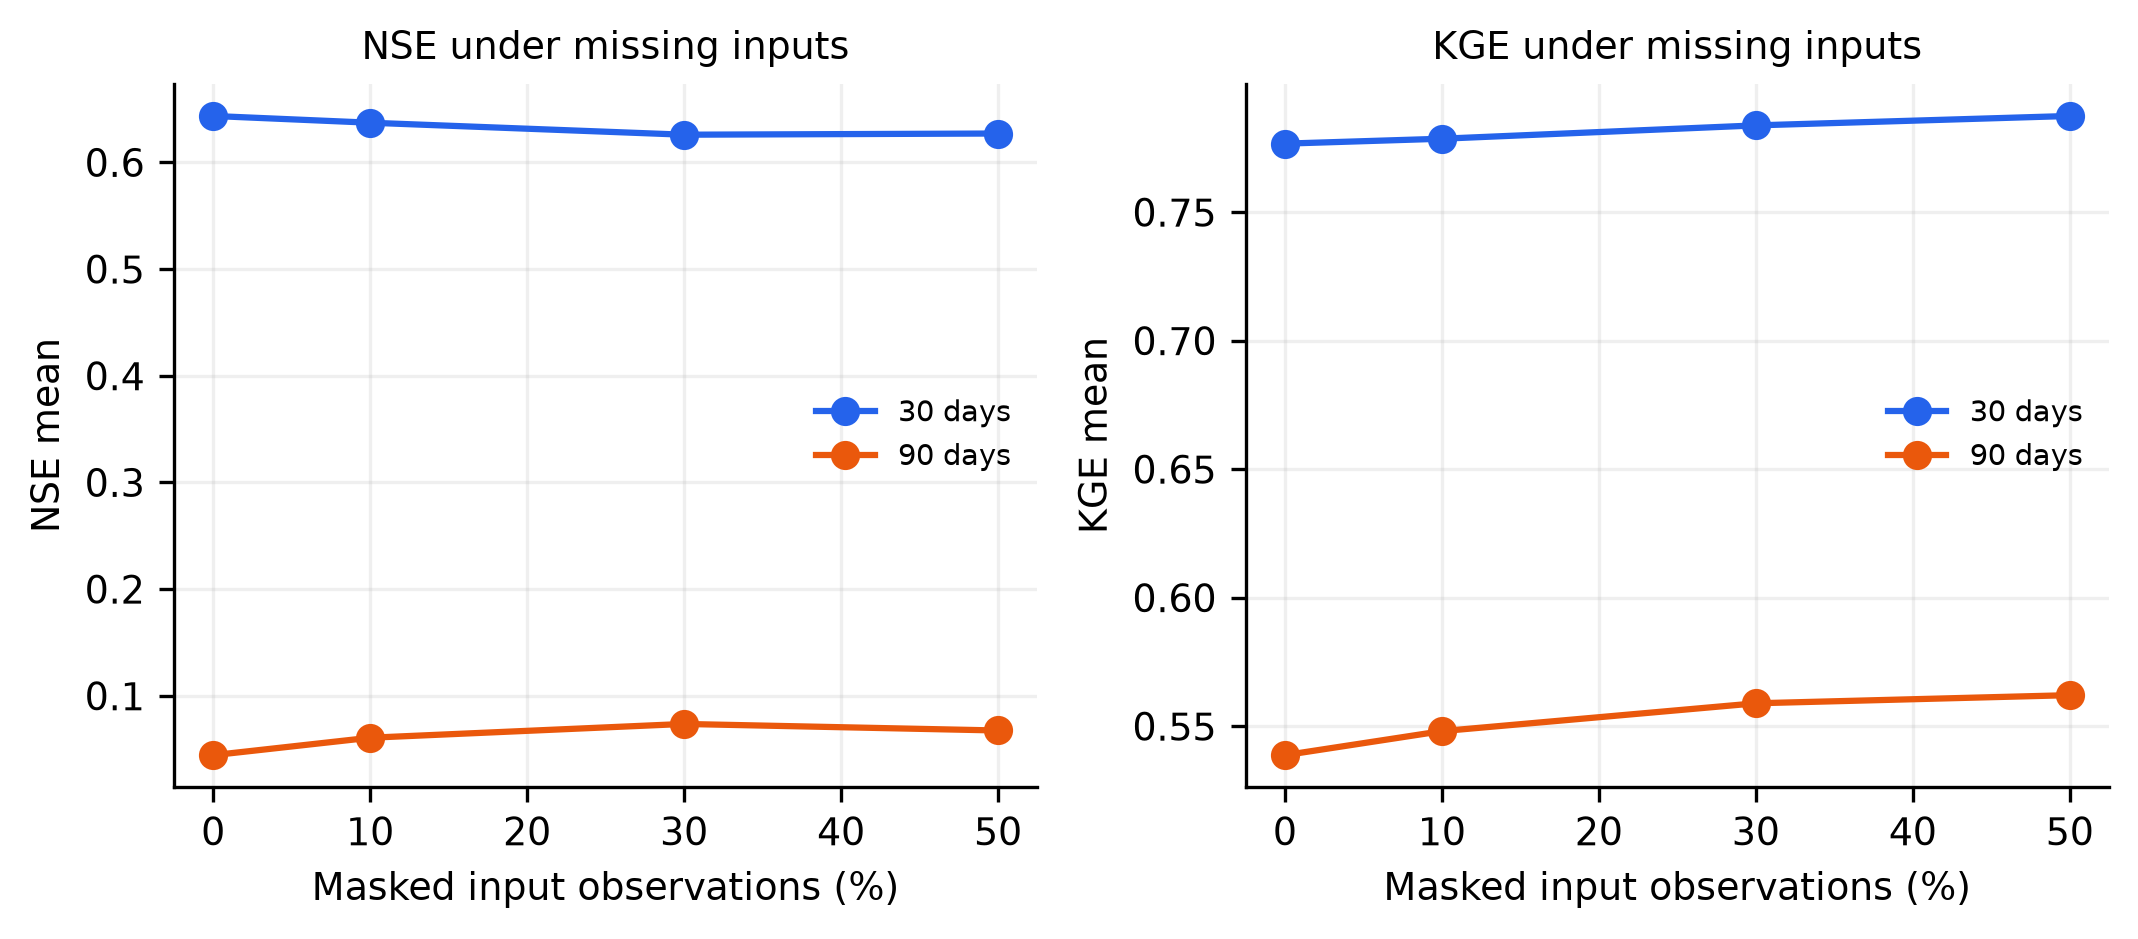
\includegraphics[width=0.8\linewidth]{figures/fig6_missingness.png}
\caption{Calibrated GRU skill under random input missingness.}
\label{fig:missing}
\end{figure}

\paragraph{Evaluation-window sensitivity.}
The training stride changes the number of training windows but not the test-day
protocol. Re-evaluating the trained models on a stride-3 test subset (matching
training) changes mean NSE from 0.575 to 0.606 at 30 days and from $-0.189$ to
$-0.197$ at 90 days across seeds; median and KGE differences are below 0.01. A
stride-7 subset gives higher 90-day mean NSE (0.033) because it excludes the
outlier, but its median and KGE remain stable. The conclusions are therefore
not driven by the stride choice.

\subsection{State-level heterogeneity}

Table~\ref{tab:states} breaks the seed-averaged per-site results down by state.
At 90 days, the median NSE is 0.545 vs $-0.165$ for persistence in Nebraska,
$-0.386$ vs $-0.526$ in California, and 0.816 vs 0.712 in Texas. The mean
improvements are smaller and not uniform: Nebraska improves modestly, California
improves slightly, and Texas (five wells) has a slightly lower mean KGE for the
model. At 30 days the model is essentially tied with persistence in California
and Texas and has a lower mean KGE in Nebraska. The aggregate result is
therefore not driven by a single state, but the gains are heterogeneous; future
benchmark reports should include state or aquifer strata.

\begin{table}[t]
\centering
\caption{Seed-averaged per-site skill by state. Values are means across wells;
model = calibrated GRU, pers = persistence. $N$ is the number of wells at 30/90
days.}
\label{tab:states}
\resizebox{\linewidth}{!}{%
\begin{tabular}{lrrrrrr}
\toprule
State & $N$ & 30d NSE (model/pers) & 30d KGE (model/pers) & 90d NSE (model/pers) & 90d KGE (model/pers) \\
\midrule
CA & 32/32 & 0.638/0.631 & 0.796/0.788 & $-0.423$/$-0.457$ & 0.413/0.379 \\
NE & 37/36 & 0.480/0.483 & 0.709/0.760 & $-0.103$/$-0.118$ & 0.550/0.479 \\
TX & 5/5 & 0.885/0.876 & 0.916/0.932 & 0.697/0.599 & 0.772/0.789 \\
\bottomrule
\end{tabular}}
\end{table}

\subsection{Outlier case}

Figure~\ref{fig:outlier} shows the well that dominates the 90-day mean error.
The full record (top) contains strong seasonal spikes consistent with pumping
cycles and a multi-year declining trend. In the available test period (bottom;
April--October 2019), the calibrated GRU predicts a smooth seasonal rise while
the observed level continues to decline; persistence follows the observations
more closely. We do not have pumping or abstraction records for this well, so
we cannot attribute the shift to a specific mechanism---pumping changes,
drought, and sensor or datum changes are all plausible. The case illustrates
why per-site outliers should be inspected rather than relying only on
aggregate means.

\begin{figure}[t]
\centering
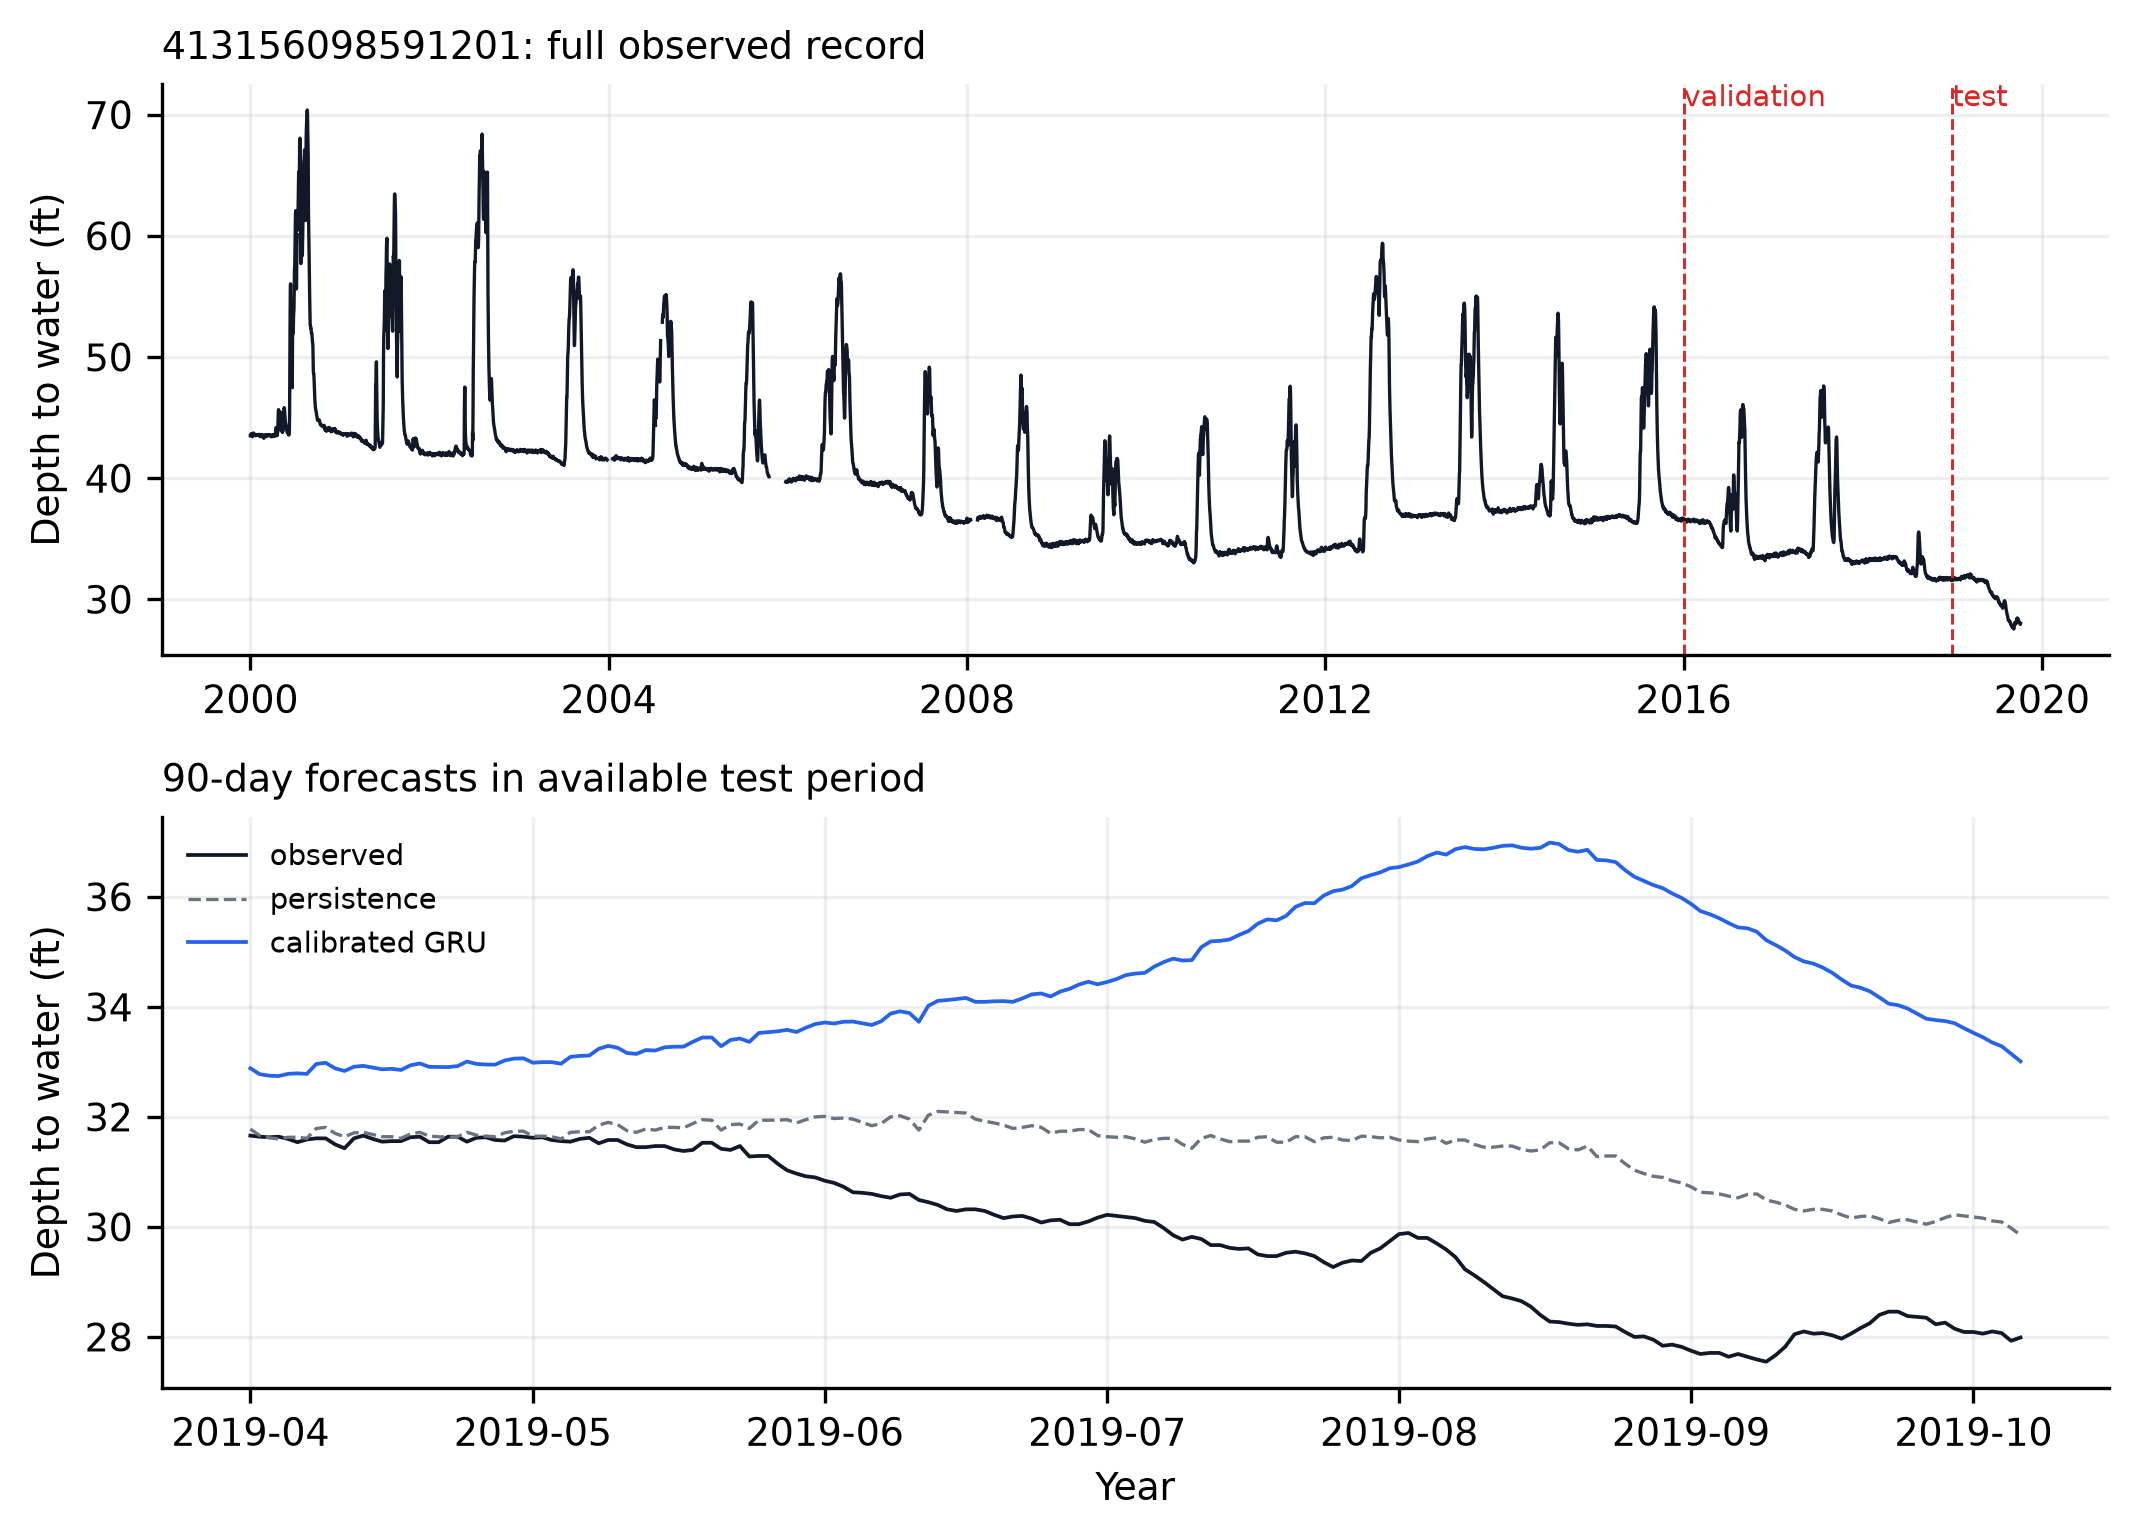
\includegraphics[width=\linewidth]{figures/fig7_outlier.png}
\caption{Outlier well \texttt{413156098591201}. Top: full observed record with
validation and test boundaries. Bottom: 90-day forecasts in the available test
period. The calibrated GRU predicts a smooth seasonal rise while the observed
level continues a multi-year decline; persistence remains closer to the
observations.}
\label{fig:outlier}
\end{figure}

\section{Discussion}

Three practical lessons emerge. First, persistence is an extremely strong
baseline for daily groundwater levels at short horizons. Studies that report
large 30-day gains should report persistence on the same temporal split; our
multi-seed analysis shows that a calibrated global GRU is statistically tied
with persistence at 30 days. Second, residual targets and per-site blending are
necessary for a global model to remain usable across heterogeneous wells. The
uncalibrated GRU's catastrophic failures are not rare edge cases: low-variance
wells are common, and a single bad well can dominate a mean metric. Third, the
useful signal appears at longer horizons. At 90 days, persistence is already
poor (mean NSE $-0.218$), and the calibrated model improves median NSE, mean
KGE, and median KGE across seeds, although mean NSE and mean KGE have
confidence intervals that include zero and one well drives much of the mean
behavior. The state-level table and the per-site win/loss counts reinforce a
more nuanced reading: the 90-day result is a distributional improvement
(median and KGE) rather than a uniform mean gain. At 90 days, 55/73 wells
improve on NSE but 13 worsen; the mean is dominated by a few wells. We
therefore recommend that benchmark users report the full distribution, not
only a mean.

The outlier well illustrates a broader evaluation issue. Calibration weights
are fitted on 2016--2018 and applied to 2019--2024; one well experiences a
validation-to-test shift that neither the GRU nor the blending weight
anticipates. This argues for reporting median metrics, win rates, and
per-site behavior alongside means, and for treating calibration as a
validation-dependent procedure whose robustness should be checked.

\subsection{Benchmark protocol and future models}

We recommend that future work on gwbench (i) use the temporal split; (ii)
report persistence on the same anchors; (iii) report mean and median NSE/KGE,
win rates, and confidence intervals; (iv) fit any calibration on validation
only; (v) inspect per-site outliers; (vi) include missing-data stress tests;
and (vii) release code and data. The current GRU is a baseline, not the
endpoint; the benchmark is designed to be extended with new models and new
regions.

\subsection{Site embeddings and unseen wells}

The current model uses a learned site embedding and is therefore evaluated on
wells seen during training. For an unseen well the embedding is undefined, so
the present results should not be interpreted as a leave-well-out transfer
test. A proper cross-site experiment requires static predictors such as well
depth, aquifer, land cover, and climate, and is left for future work; the
benchmark repository includes the split machinery needed for that study.

\subsection{Climate covariates and physical limits}

The model is univariate apart from calendar features. It cannot represent
recharge, pumping, evapotranspiration, or storage changes; at 90 days these
omissions likely limit absolute skill. Adding precipitation, potential
evapotranspiration, and GRACE-derived storage anomalies is the most promising
route to improving the 90-day ceiling. The gains reported here come from
persistence anchoring and validation calibration, not from external drivers.

\subsection{Limitations}

The benchmark covers three states and one parameter/statistic; the clean core
has 74 wells. The calibration weight is fitted on a single validation period,
and performance can degrade under distribution shift. USGS records contain
datum and sensor changes that we flag and filter but do not physically correct.
The univariate design and site-embedding limitation are discussed above and
define the main directions for future work.

\section{Conclusions}

We presented \texttt{gwbench}, a reproducible public-data benchmark for daily
groundwater-level forecasting, and a persistence-anchored residual GRU with
per-site calibration. At 30 days, the calibrated model is statistically tied
with persistence on mean NSE; at 90 days, it improves median NSE from $-0.181$
to 0.267 (95\% CI for the median gain 0.033--0.207) and mean KGE from 0.456 to
0.505, although mean NSE and mean KGE confidence intervals include zero and
one distribution-shift well dominates the mean. The uncalibrated GRU
fails catastrophically on low-variance wells, and the validation-fitted
blending weight is essential. The model is also stable under 10--50\% missing
input observations. We hope the benchmark encourages stronger baselines,
temporal splits, and per-site reporting in groundwater ML.

\section*{Data and code availability}

All raw observations are public USGS NWIS data \citep{usgs2026}. Code,
experiment configurations, and figure-generation scripts are available at
\url{\codeurl}. Processed panels and the release archive are archived at
\href{https://doi.org/10.5281/zenodo.23749304}{\mbox{\texttt{10.5281/zenodo.23749304}}}.
The 30-day, 90-day, and seed-study Kaggle notebooks are
available at \url{\kaggleurl},
\url{https://www.kaggle.com/code/kkksssaaalzy/gwbench-gru-h90}, and
\url{https://www.kaggle.com/code/kkksssaaalzy/gwbench-seeds}; the public
Kaggle dataset is available at
\url{https://www.kaggle.com/datasets/kkksssaaalzy/gwbench-data}.

\section*{CRediT authorship contribution statement}

\textbf{Zhaoyang Li:} Conceptualization, Data curation, Formal analysis,
Investigation, Methodology, Software, Validation, Visualization, Writing --
original draft, Writing -- review and editing.

\section*{Declaration of competing interest}

The authors declare that they have no known competing financial interests or
personal relationships that could have appeared to influence the work
reported in this paper.

\section*{Acknowledgements}

The author thanks the U.S. Geological Survey for maintaining the NWIS
database and Kaggle for providing GPU resources used in the experiments.

\bibliographystyle{elsarticle-num}
\bibliography{refs}

\end{document}
